\section{Ablation Study}
\begin{figure}[t]
  \centering
  \begin{subfigure}{0.3\linewidth}
    \centering
    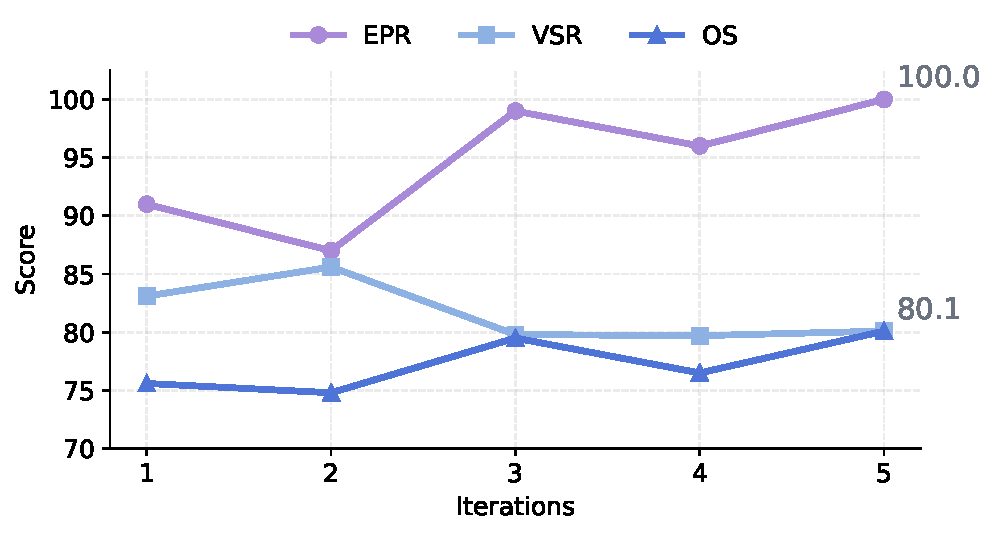
\includegraphics[width=\linewidth]{figures/ablation_iter_line.pdf}
    \caption{Iterations Ablation}
    \label{fig:abl-iter}
  \end{subfigure}\hfill
  \begin{subfigure}{0.3\linewidth}
    \centering
    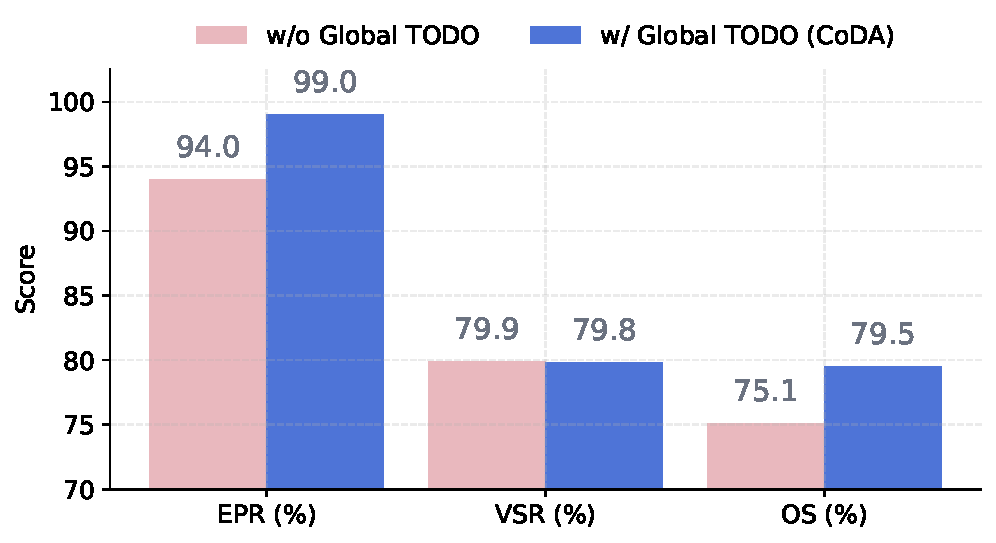
\includegraphics[width=\linewidth]{figures/ablation_globalTODO_metrics.pdf}
    \caption{Global TODO Ablation}
    \label{fig:abl-todo}
  \end{subfigure}\hfill
  \begin{subfigure}{0.3\linewidth}
    \centering
    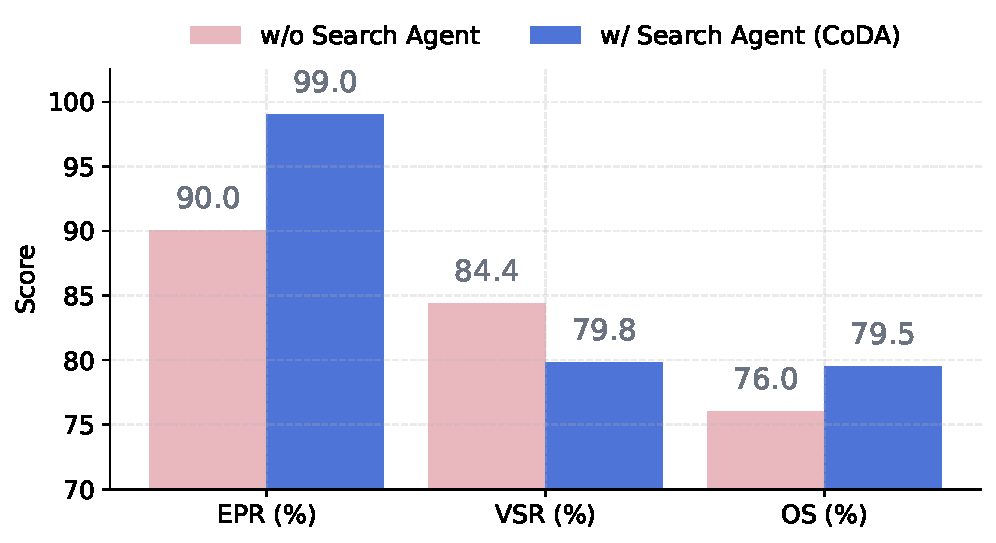
\includegraphics[width=\linewidth]{figures/ablation_search_metrics.pdf}
    \caption{Search Agent Ablation}
    \label{fig:abl-search}
  \end{subfigure}
  \caption{Ablation results. (a): Performance (EPR, VSR, OS) across different iteration counts. (b) Comparison of EPR, VSR, and OS with vs. without Global TODO. (c) Comparison of EPR, VSR, and OS with vs. without the Search Agent.}
  \label{fig:ablation-three}
\end{figure}

To validate the contributions of key components in \methodname{}, we conduct controlled ablation experiments on the MatplotBench dataset, using \io{gemini-2.5-pro} as the backbone. 
These studies isolate the impact of (1) iterative self-reflection through refinement loops, (2) the global TODO list for high-level planning, and (3) the Search Agent for code example retrieval. 
All ablations maintain the core multi-agent pipeline but adjust the specified components. 
This analysis not only confirms the necessity of each feature but also provides insights into design trade-offs, such as accuracy-efficiency balances, highlighting \methodname{}'s principled architecture for robust, autonomous visualization.
We evaluate the impact of these components on the OS metric. Figure~\ref{fig:ablation-three} summarizes the findings.





\subsection{Impact of Self-Evolution}



Figure~\ref{fig:ablation-three} shows that OS generally improves with additional iterations, from 75.6\% at 1 iteration to 79.5\% at 3 iterations (\methodname{} default), with further gains to 80.1\% at 5 iterations, though with fluctuations and marginal benefits beyond 3 (+0.6\% in OS from 3 to 5).
EPR surges by 8.0\% from 1 to 3 iterations due to robust initial code generation by the Code Generator, stabilizing near 100\% thereafter. VSR fluctuates initially but converges around 80\%, as the Visual Evaluator identifies and refines subtle mismatches in data mappings and aesthetics. 
Beyond 3 iterations, latency increases without proportional accuracy benefits, validating our lightweight configuration optimization that tunes limits based on validation performance. 
With minimal iterations, performance degrades toward baseline levels, emphasizing that shallow, one-shot generation fails in messy environments.

\subsection{Role of Global TODO List}

The global TODO list, generated by the Query Analyzer, serves as a high-level blueprint for task decomposition and routing, ensuring coherence across agents.
We ablate this by replacing it with understanding-query-only prompts (no structured decomposition).
As shown in Figure~\ref{fig:ablation-three}, removing the global TODO list yields a stark drop in OS to 75.1\% (-4.4\% absolute), 
with EPR falling by 5.0\% due to fragmented intent extraction, e.g., the VizMapping Agent selects suboptimal chart types without cross-referencing subtasks like ``highlight peaks.''
VSR remains stable, indicating that visual quality is less dependent on global planning, but overall success suffers from incomplete workflows, such as unaddressed statistical insights from the Data Processor. 
This confirms the value of structured planning in agentic workflows, where it prevents the noise of unstructured agent interactions.

\subsection{Effectiveness of Example Search Agent}
The Search Agent retrieves relevant plotting code examples (e.g., from Matplotlib repositories) to inspire the Builder Agent, addressing LLM limitations in recalling domain-specific syntax. We study this by disabling retrieval, relying solely on the backbone LLM's internal knowledge.
Figure~\ref{fig:ablation-three} reveals that without the Search Agent, OS declines to 76.0\% (-3.5\%), 
primarily due to a 9.0\% drop in EPR from syntactic errors in specialized visualizations (e.g., custom subplots). 
Enabling code search improves accuracy by providing ranked snippets, grounding LLM agents' coding knowledge to specific problems. This ablation highlights the extensibility of \methodname{}, where external inspiration bridges gaps in LLM training data, making the system more reliable without post-training.



